\begin{frame}{Knowledge Acquisition}

    \begin{figure} [H]
        \begin{center}
            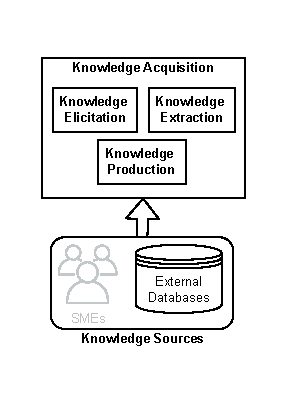
\includegraphics[scale=0.8]{images/KGBS-knowledge-acquisition.pdf} 
            \caption{KGBS: Knowledge acquisition} 
        \end{center}
    \end{figure}

\end{frame}

% \begin{frame}{Knowledge modeling}

%     \begin{figure} [H]
%         \begin{center}
%             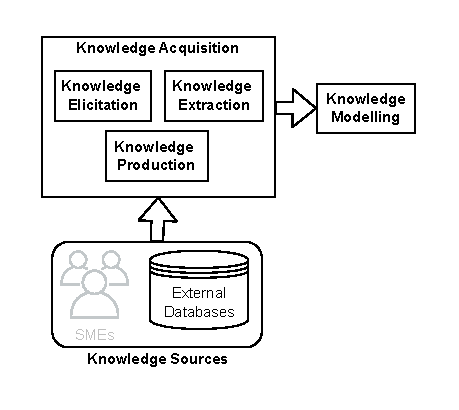
\includegraphics[scale=0.8]{images/KGBS-knowledge-modelling.pdf} 
%             \caption{KGBS: Knowledge modeling} 
%         \end{center}
%     \end{figure}

% \end{frame}

\begin{frame}{Knowledge Graph}

    \begin{figure} [H]
        \begin{center}
            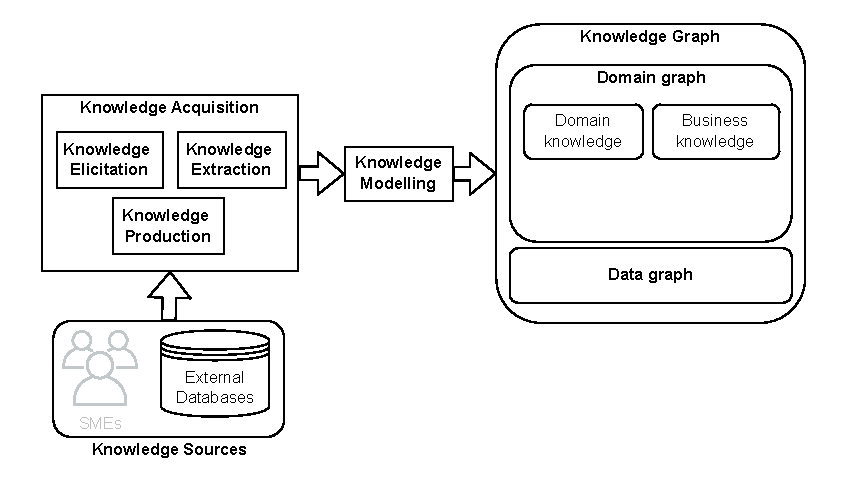
\includegraphics[scale=0.6]{images/KGBS-knowledge-modelling-kg.pdf} 
            \caption{KGBS: Knowledge Graph} 
        \end{center}
    \end{figure}

\end{frame}

\begin{frame}{Knowledge consumption}

    \begin{figure} [H]
        \begin{center}
            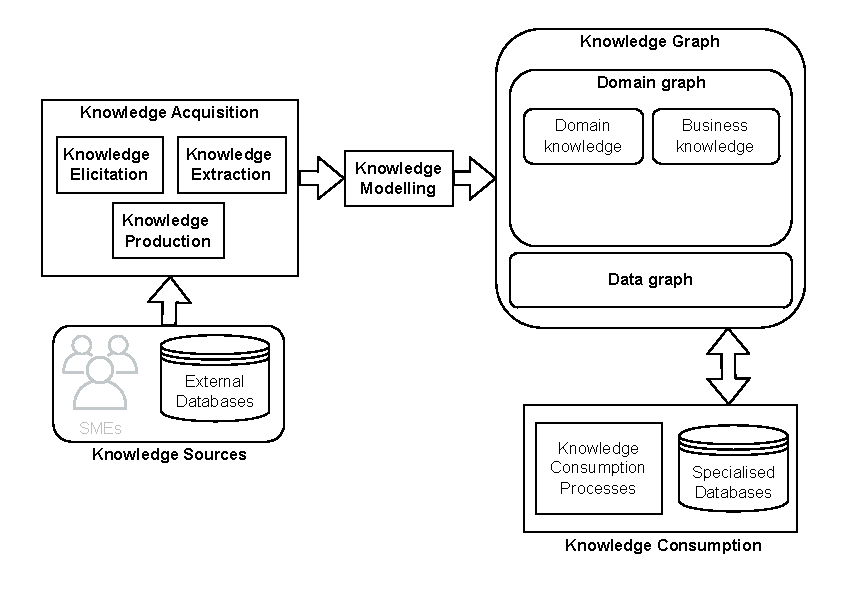
\includegraphics[scale=0.6]{images/KGBS-knowledge-consumption.pdf} 
            \caption{KGBS: knowledge consumption} 
        \end{center}
    \end{figure}

\end{frame}

\begin{frame}{Knowledge Graph-Based System architecture}

    \begin{figure} [H]
        \begin{center}
            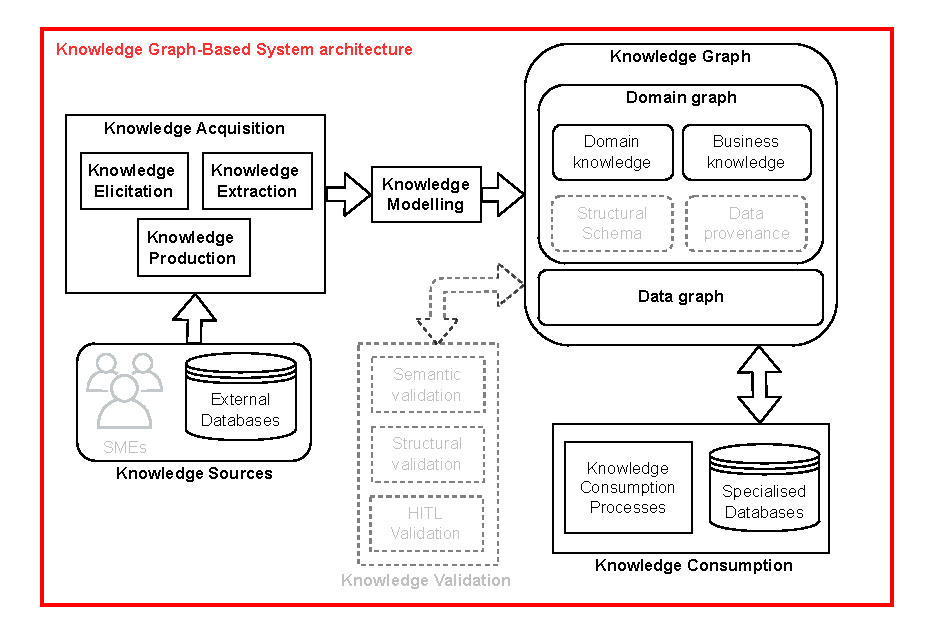
\includegraphics[scale=0.5]{images/KGBS-architecture.pdf} 
            \caption{KGBS architecture} 
        \end{center}
    \end{figure}

\end{frame}

% \begin{frame}{Knowledge Graph vs Ontology}

%     \begin{figure} [H]
%         \begin{center}
%             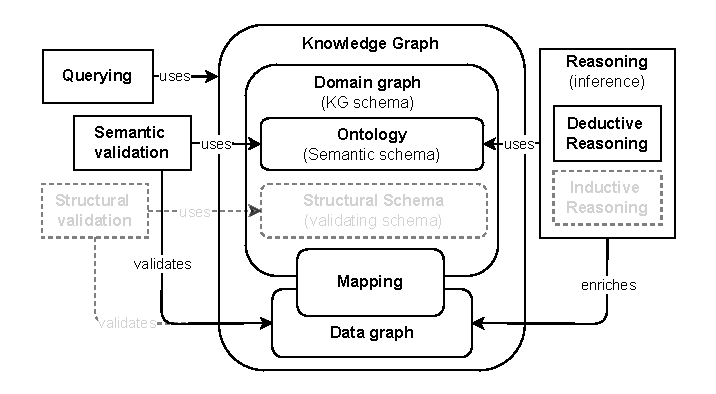
\includegraphics[scale=0.8]{images/kg-def-simple.pdf} 
%             \caption{Knowledge Graph definition} 
%         \end{center}
%     \end{figure}

% \end{frame}

\section{Contributions}

\begin{frame}{Ontology Learning Applied Framework (OLAF)}

    \begin{figure} [H]
        \begin{center}
            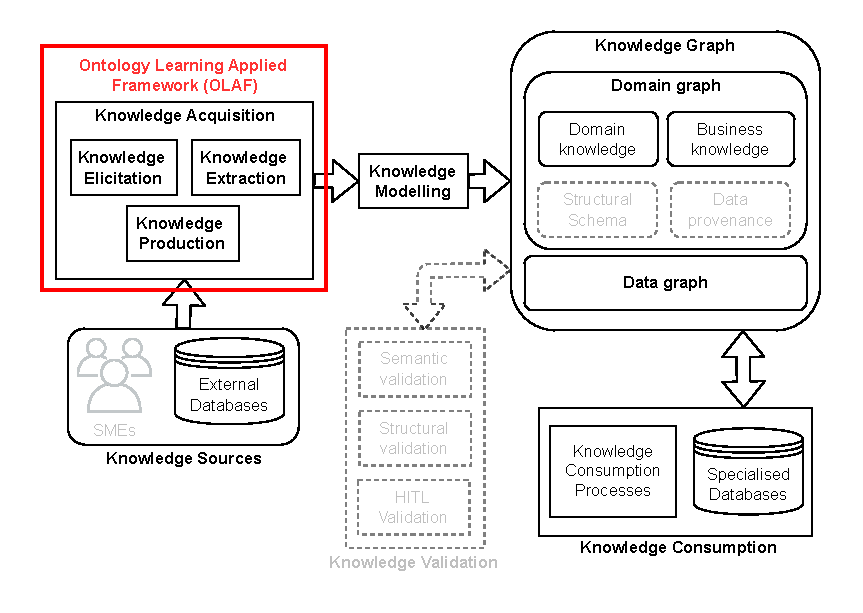
\includegraphics[scale=0.5]{images/KGBS-knowledge-acquisition-OLAF.pdf} 
            \caption{KGBS architecture: OLAF} 
        \end{center}
    \end{figure}

\end{frame}

\begin{frame}{Information Retrieval ontology}

    \begin{figure} [H]
        \begin{center}
            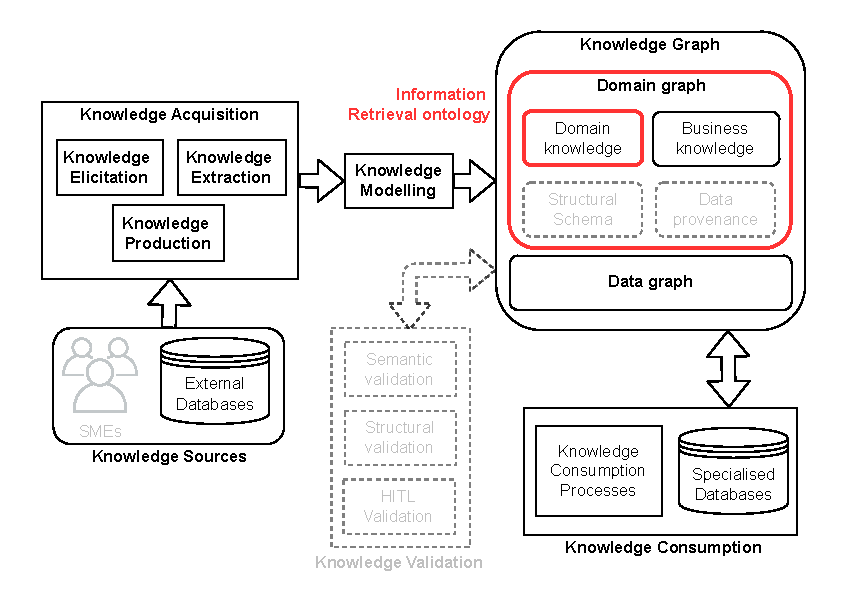
\includegraphics[scale=0.5]{images/KGBS-knowledge-modelling-kg-IR-onto.pdf} 
            \caption{KGBS architecture: IR ontology} 
        \end{center}
    \end{figure}

\end{frame}

\begin{frame}{KG-based Information Retrieval}

    \begin{figure} [H]
        \begin{center}
            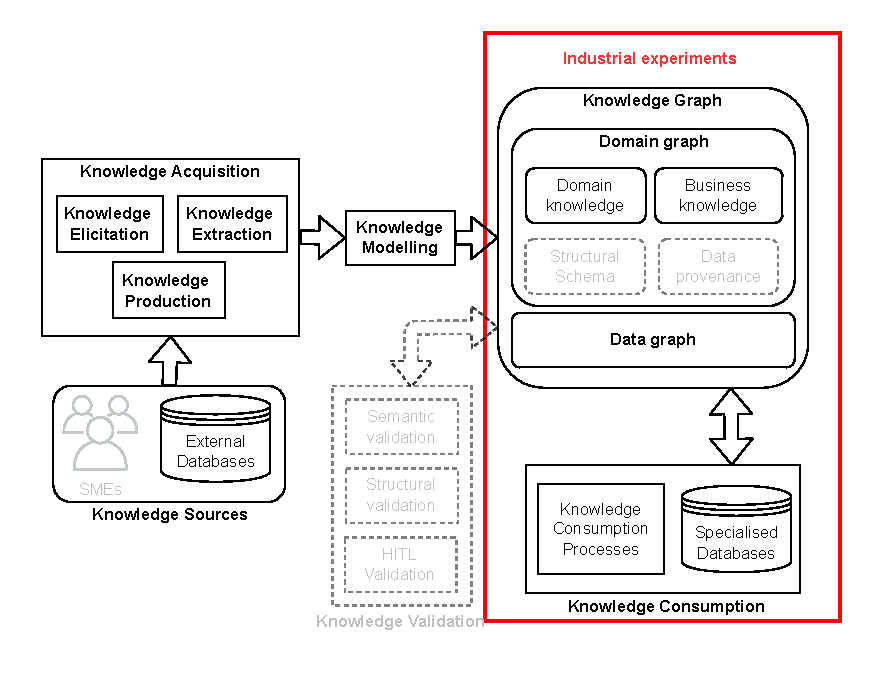
\includegraphics[scale=0.5]{images/KGBS-knowledge-consumption-industrial-exp.pdf} 
            \caption{KGBS architecture: Industrial experiments} 
        \end{center}
    \end{figure}

\end{frame}

\begin{frame}{In this presentation}

    \begin{figure} [H]
        \begin{center}
            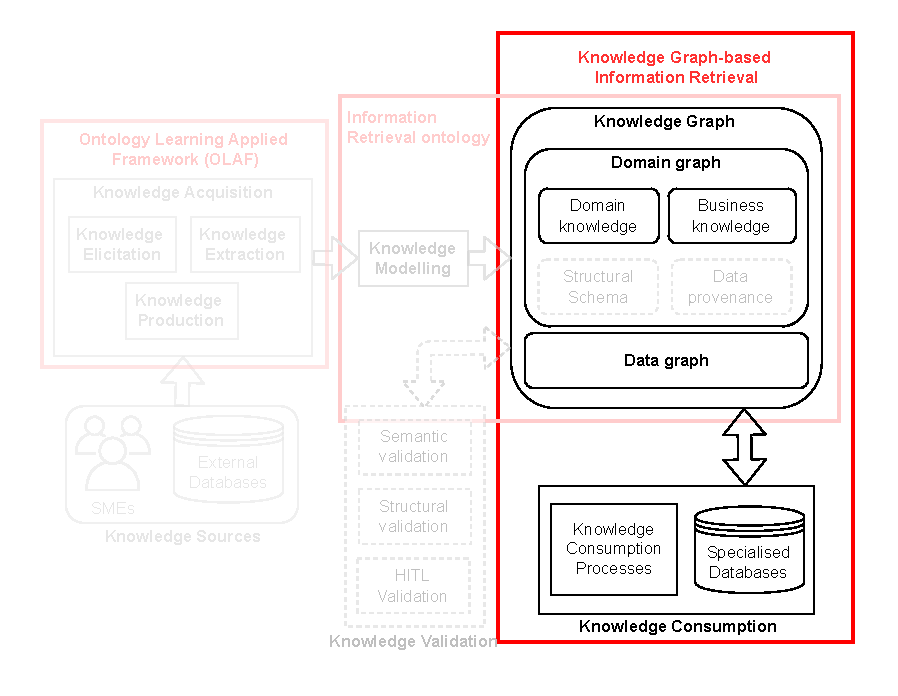
\includegraphics[scale=0.5]{images/KGBS-architecture-focus-TP-expe.pdf} 
            \caption{This presentation KGBS architecture components focus} 
        \end{center}
    \end{figure}

\end{frame}